\documentclass[11pt]{report}
\usepackage{fullpage}
%\usepackage{sourcesanspro, sourcecodepro}
\usepackage{minted}
\usepackage{graphicx}
\usepackage{awesomebox}
\usepackage{hyperref}
\usepackage{float} % stops images from moving around
\usepackage[a4paper, total={6in, 8in}, margin=0.75in]{geometry}
\usepackage{etoolbox}
\makeatletter
\patchcmd{\chapter}{\if@openright\cleardoublepage\else\clearpage\fi}{}{}{}
\RequirePackage[T1]{fontenc}
\RequirePackage[default,light,black]{roboto}

\hypersetup{
    colorlinks=true,
    linkcolor=blue,
    citecolor=blue,
    filecolor=blue,
    urlcolor=blue,
    pdfborder={0 0 0}
}

\graphicspath{{./images/}}

\title{APSC 258: Lab 5 Manual}
\author{Andre Cox}

\begin{document}
\maketitle
\tableofcontents

\clearpage

\chapter{Introduction}
\section{Introducing the Convolution Layer}
In our last lab you got to work with dense layers. You may have noticed that the neural network was not very effective. In this lab we will introduce the concept of Convolution layers. To explain why we use these layers we must first revisit the concept of a dense layer. You can think of a dense layer as a layer of neurons. The neurons in a dense layer are simply a weighted sum of the inputs. When training the neural network these weights get adjusted until the network is able to predict the correct output. This is a great way to predict simple things such as the average grade a student may achieve based on class attendance and the amount of homework they have done. However they become less effective as the number and complexity of the inputs increase. For instance let's say we have an image of our track that we feed into a dense layers. These dense layers may be able to predict the steering angle of the car however they could get confused depending on the different features of the image. This is because these layers represent the image in 1 dimension. Let me give you an example. 

\begin{figure}[h]
\centering
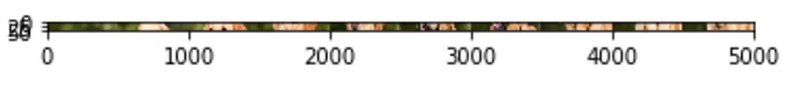
\includegraphics[width=0.8\textwidth]{./images/dogdense.png}
\caption{A 1D representation of an image}
\label{fig:1d}
\end{figure}

Can you tell what this above image is? Probably not easily, this is essentially what our neural network has to process with dense layers. We need a way to represent the image in a 2 dimensional space.

\begin{figure}[h]
\centering
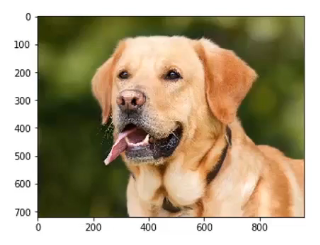
\includegraphics[width=0.5\textwidth]{./images/dogconv.png}
\caption{A 2D representation of an image}
\label{fig:2d}
\end{figure}
You can see that the image is now represented in a 2 dimensional space and is now much easier to understand. This is why convolution layers are so useful. 

\section{More on Convolution Layers}
Convolution layers are useful for feature extraction. For instance if we were running facial recognition we would use multiple layers that would each progressively extract features with more and more detail. An example of this is shown below.

\begin{figure}[h]
\centering
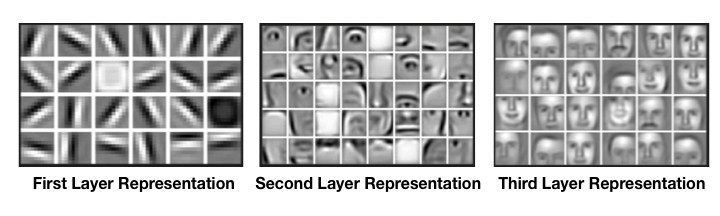
\includegraphics[width=0.8\textwidth]{./images/featureextraction.jpg}
\caption{Extracting features from an image}
\label{fig:conv1}
\end{figure}

Once we have extracted our features we can use a Flatten layer to turn the extracted features back into a 1 dimensional vector. Then this can be used as input to a dense layer. A representation of this is shown below. You can see that there is also a pooling layer all that does is reduce the size of the image. This is useful for increasing the efficiency of the network. 

\begin{figure}[h]
\centering
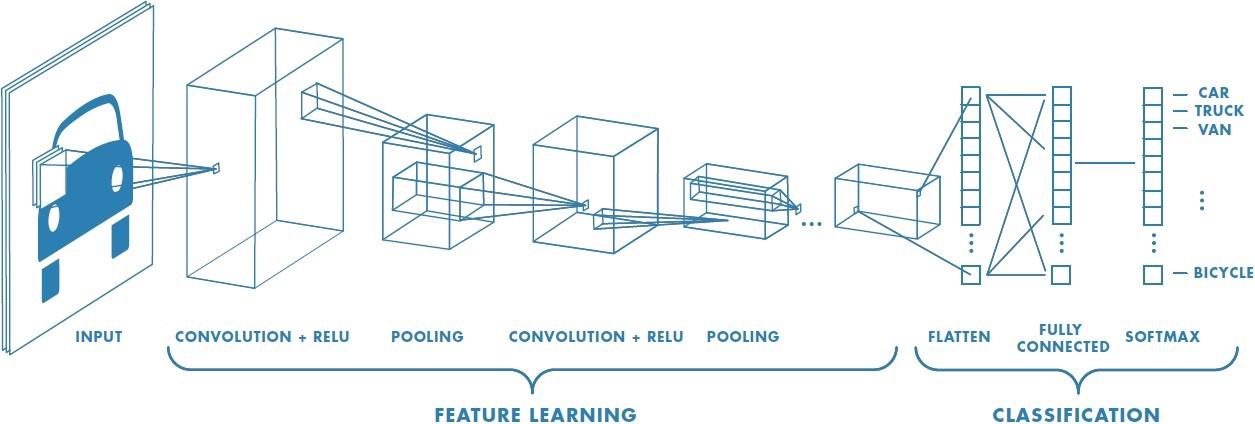
\includegraphics[width=0.8\textwidth]{./images/convexamp.jpeg}
\caption{Representation of a CNN}
\label{fig:cnn}
\end{figure}

\clearpage

\chapter{Using the Convolution Layer}
Now that we have a better understanding of the convolution layer we can use it in our neural network.
\section{Creating a Convolution Layer}
Below is a simple example of a convolutional neural network. Where all the parameters are explained.
\begin{minted}[linenos, fontfamily=courier, style=monokai, bgcolor=black, breaklines]{python} 
    from keras.layers import Conv2D, MaxPooling2D, Dense Sequential, InputLayer, Flatten
    # a sequential model is a model that is made up of layers
    model = Sequential()
    # the input layer is the first layer in the model
    model.add(InputLayer(input_shape=(100, 66, 1)))

    # the convolution layer
    # the different parameters are:
    # the number of output filters: 32
    # the kernel size: (3, 3) specifying the height and width of the 2D convolution window.
    # the activation function: ReLU the type of activation function that is used in the convolution layer.
    model.add(Conv2D(32, kernel_size=(3, 3), activation='relu'))

    # the pooling layer
    # the pooling layer is used to reduce the size of the image.
    # the pool size: (2, 2) specifying the height and width of the 2D pooling window.
    model.add(MaxPooling2D(pool_size=(2, 2)))

    # the flatten layer
    # the flatten layer is used to turn the output of the convolution layer into a 1 dimensional vector.
    model.add(Flatten())

    # our dense layers, used to do the classification
    model.add(Dense(100, activation='relu'))
    model.add(Dense(50, activation='relu'))
    model.add(Dense(10, activation='relu'))
    model.add(Dense(1, activation='relu'))
\end{minted}

\chapter{Applying the Convolution Layer}
Now that you have a good grasp of the convolution layer we can apply it to our neural network. Open the model from your previous lab and add try experimenting by adding the convolution layer to the model. See if multiple convolution layers function better than a single one. Once you are done with this and are happy with your model you can save the model and download it. Then you can run the model with the following code.
"python runNetwork.py -m yourConvolutionModel.h5"

\notebox{
    \textbf{Roadblock:}
    You may have noticed that while your training model has a very low mean squared error, while your testing model has a very high mean squared error. This is caused by overfitting. Overfitting is when the model is too complex and cannot generalize to new data. This is a problem that we will solve in the next lab.
}


\end{document}